\documentclass[tikz,border=10pt]{standalone}
\usepackage{pgfplots}
\usepgfplotslibrary{fillbetween}
\pgfplotsset{compat=1.18}

\begin{document}

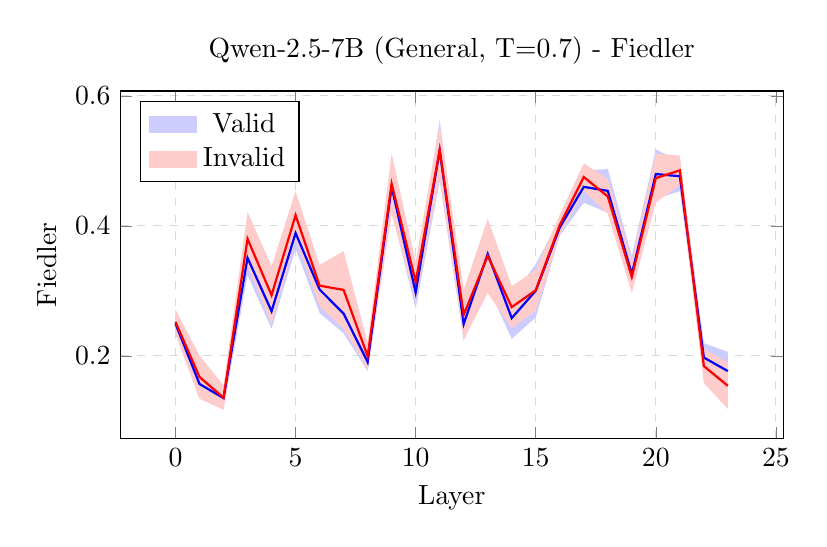
\begin{tikzpicture}
\pgfplotstableread[row sep=newline, col sep=comma]{
layer,v_mean,v_std,i_mean,i_std,v_upper,v_lower,i_upper,i_lower

0,0.249455136,0.01559963017880058,0.25208854300000005,0.01915366706762224,0.2650547661788006,0.2338555058211994,0.2712422100676223,0.23293487593237783

1,0.15663476325,0.02252408515335162,0.167366735,0.03311521637722365,0.1791588484033516,0.1341106780966484,0.20048195137722363,0.13425151862277634

2,0.1349360750625,0.017173179873164444,0.1355252172,0.01873088716191518,0.15210925493566443,0.11776289518933555,0.15425610436191517,0.11679433003808481

3,0.350629519375,0.026642795809515986,0.3798331965,0.04173657371033434,0.377272315184516,0.32398672356548397,0.42156977021033437,0.3380966227896657

4,0.26856630137500004,0.026932749960820526,0.29331379450000006,0.0444701850795761,0.29549905133582055,0.24163355141417953,0.3377839795795762,0.24884360942042397

5,0.388840571875,0.02389640912318324,0.4163139105,0.036954255194767985,0.41273698099818323,0.36494416275181674,0.45326816569476797,0.379359655305232

6,0.302011399,0.036211458669069,0.3078885445,0.03185739647237877,0.338222857669069,0.265799940330931,0.3397459409723788,0.27603114802762124

7,0.264893629,0.030223985952467097,0.30139729200000004,0.059794220324741625,0.29511761495246713,0.23466964304753293,0.36119151232474167,0.2416030716752584

8,0.190382189125,0.013811278701900217,0.1994392275,0.02017149303083122,0.2041934678269002,0.17657091042309978,0.21961072053083122,0.1792677344691688

9,0.45993546399999996,0.03807866458373011,0.464808263,0.04684562900621932,0.49801412858373006,0.42185679941626986,0.5116538920062194,0.4179626339937807

10,0.297379486125,0.024636644799854467,0.31410237550000003,0.030431948045520303,0.3220161309248544,0.27274284132514554,0.3445343235455203,0.28367042745447973

11,0.516136895875,0.04679084622646457,0.5167070085000001,0.040473948818714994,0.5629277421014646,0.46934604964853543,0.5571809573187151,0.47623305968128504

12,0.249005390875,0.0256207848351231,0.26321143399999997,0.03855636665944336,0.2746261757101231,0.22338460603987692,0.3017678006594433,0.2246550673405566

13,0.35669106775,0.05003197414296012,0.35376856300000004,0.05718142488782433,0.4067230418929601,0.30665909360703986,0.4109499878878244,0.2965871381121757

14,0.25797769800000003,0.03189368685191886,0.2748892095,0.0322792702501568,0.2898713848519189,0.2260840111480812,0.3071684797501568,0.2426099392498432

15,0.300126637875,0.04097588447020381,0.300862297,0.03153833921035143,0.3411025223452038,0.2591507534047962,0.33240063621035143,0.26932395778964857

16,0.39745134887499994,0.012492927991715344,0.40121289749999994,0.01585984043276698,0.4099442768667153,0.3849584208832846,0.41707273793276695,0.38535305706723294

17,0.45993663625,0.024344980614817432,0.4750609914999999,0.021105293185618344,0.4842816168648174,0.43559165563518254,0.49616628468561824,0.4539556983143816

18,0.453792968125,0.033720209878932525,0.4451779995,0.02694420289465983,0.4875131780039325,0.42007275824606743,0.4721222023946598,0.41823379660534016

19,0.3258684665,0.02721921813178222,0.3211888215,0.024405539958561023,0.35308768463178225,0.29864924836821777,0.34559436145856104,0.29678328154143896

20,0.47968906462499994,0.037910031652044554,0.4734163345,0.037537447641845315,0.5175990962770445,0.4417790329729554,0.5109537821418453,0.4358788868581547

21,0.476262152375,0.023009321501398405,0.48532405800000006,0.022706880666704853,0.4992714738763984,0.45325283087360163,0.5080309386667049,0.4626171773332952

22,0.197241110375,0.022063005345548118,0.184040578,0.02630950392934494,0.21930411572054812,0.17517810502945189,0.21035008192934496,0.15773107407065506

23,0.176410795625,0.029585364369141207,0.15372981175,0.03549792538268062,0.20599615999414123,0.14682543125585878,0.18922773713268062,0.11823188636731938

}\mydata

\begin{axis}[
    width=10cm, height=6cm,
    xlabel={Layer},
    ylabel={Fiedler},
    title={Qwen-2.5-7B (General, T=0.7) - Fiedler},
    legend pos=north west,
    grid=major,
    grid style={dashed, gray!30}
]

\addplot [name path=v_upper, draw=none, forget plot] table [x=layer, y=v_upper] {\mydata};
\addplot [name path=v_lower, draw=none, forget plot] table [x=layer, y=v_lower] {\mydata};
\addplot [blue!20] fill between [of=v_upper and v_lower];

\addplot [name path=i_upper, draw=none, forget plot] table [x=layer, y=i_upper] {\mydata};
\addplot [name path=i_lower, draw=none, forget plot] table [x=layer, y=i_lower] {\mydata};
\addplot [red!20] fill between [of=i_upper and i_lower];

\addplot [blue, thick] table [x=layer, y=v_mean] {\mydata};
\addlegendentry{Valid}
\addplot [red, thick] table [x=layer, y=i_mean] {\mydata};
\addlegendentry{Invalid}

\end{axis}
\end{tikzpicture}
\end{document}
